% Chương 3: Thiết kế mức khái niệm
\chapter{THIẾT KẾ MỨC KHÁI NIỆM}

Chương này xác định các thực thể chính của hệ thống từ những yêu cầu chức năng đã trình bày ở Chương 2. Các thực thể được chia thành từng nhóm nghiệp vụ và mô tả ngắn gọn trong các bảng dưới đây.

\section{Tài khoản và phân quyền}

Nhóm thực thể này quản lý thông tin người dùng, vai trò và quyền truy cập trong hệ thống.

\begin{longtable}{p{4cm}p{9.5cm}}
\toprule
\textbf{Thực thể} & \textbf{Mô tả} \\
\midrule
\endhead
\entity{users} & Lưu tài khoản và thông tin cơ bản của người dùng. \\
\entity{roles} & Lưu danh mục vai trò của người dùng trong hệ thống. \\
\entity{permissions} & Lưu danh mục các quyền được phép thực hiện. \\
\entity{user_roles} & Liên kết người dùng với các vai trò được gán. \\
\entity{role_permissions} & Liên kết vai trò với các quyền tương ứng. \\
\bottomrule
\end{longtable}

\section{Film Lab và danh mục dịch vụ}

Nhóm thực thể này biểu diễn Film Lab, các dịch vụ và các gói dịch vụ cung cấp cho khách hàng.

\begin{longtable}{p{4cm}p{9.5cm}}
\toprule
\textbf{Thực thể} & \textbf{Mô tả} \\
\midrule
\endhead
\entity{film_labs} & Lưu hồ sơ, thông tin liên hệ và trạng thái hoạt động của Film Lab. \\
\entity{lab_services} & Lưu các dịch vụ tráng phim, scan, in ảnh và các dịch vụ khác của từng Film Lab. \\
\entity{service_packages} & Lưu các gói dịch vụ do Film Lab cung cấp. \\
\entity{package_services} & Lưu các dịch vụ thành phần và số lượng tương ứng trong mỗi gói. \\
\bottomrule
\end{longtable}

\begin{figure}[p]
    \centering
    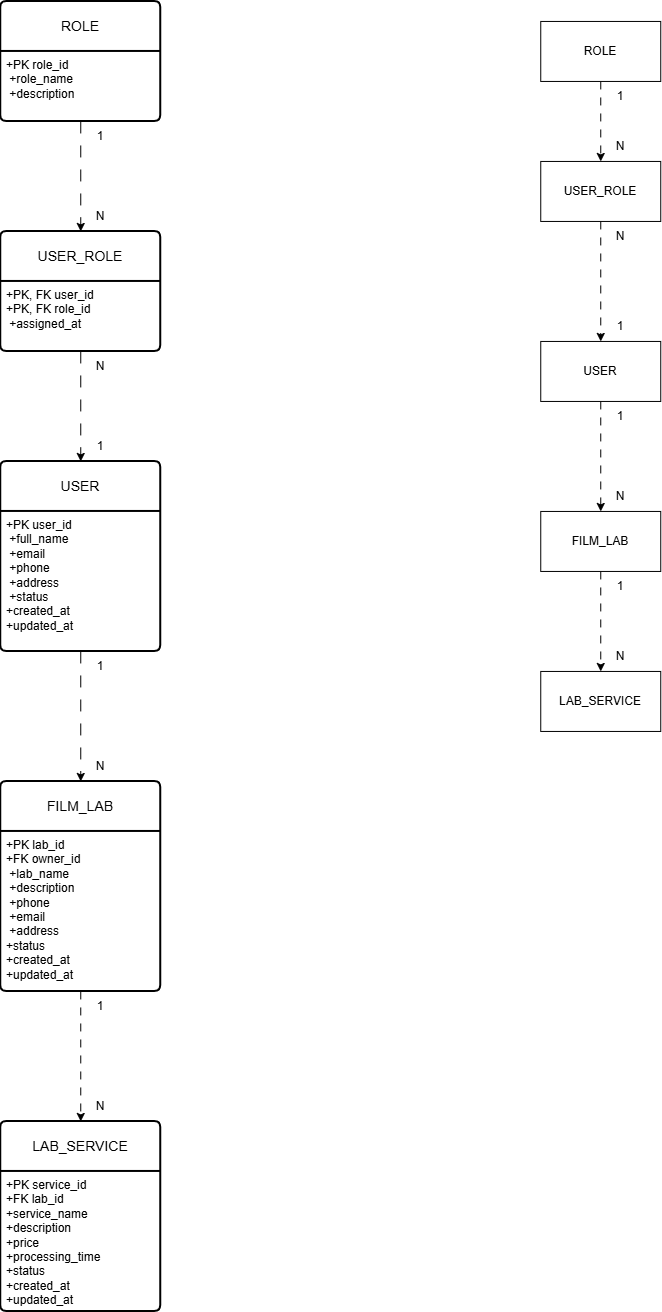
\includegraphics[width=\linewidth,height=0.82\textheight,keepaspectratio]{figures/ERD_P2.png}
    \caption{Sơ đồ thực thể tài khoản, phân quyền, Film Lab và dịch vụ}
    \label{fig:erd-account-lab}
\end{figure}
\clearpage

\section{Đơn hàng và quá trình xử lý phim}

Nhóm thực thể này quản lý đơn đặt dịch vụ, cuộn phim và lịch sử các công đoạn xử lý tại Film Lab.

\begin{longtable}{p{4cm}p{9.5cm}}
\toprule
\textbf{Thực thể} & \textbf{Mô tả} \\
\midrule
\endhead
\entity{orders} & Lưu thông tin chung của đơn đặt dịch vụ giữa khách hàng và Film Lab. \\
\entity{order_items} & Lưu từng dịch vụ hoặc gói dịch vụ được chọn trong đơn hàng. \\
\entity{film_rolls} & Lưu thông tin các cuộn phim thuộc đơn hàng. \\
\entity{processing_stages} & Lưu danh mục các công đoạn trong quy trình xử lý phim. \\
\entity{stage_logs} & Ghi nhận việc thực hiện từng công đoạn đối với mỗi cuộn phim. \\
\entity{order_status_history} & Lưu lịch sử thay đổi trạng thái của đơn hàng. \\
\entity{pickup_delivery_requests} & Lưu yêu cầu nhận phim hoặc giao trả phim của đơn hàng. \\
\bottomrule
\end{longtable}

\section{Kho ảnh phim số}

Nhóm thực thể này quản lý file scan, thông tin mô tả ảnh và cách người dùng tổ chức bộ sưu tập ảnh phim số.

\begin{longtable}{p{4cm}p{9.5cm}}
\toprule
\textbf{Thực thể} & \textbf{Mô tả} \\
\midrule
\endhead
\entity{scan_files} & Lưu vị trí, định dạng, kích thước và trạng thái của file ảnh scan. \\
\entity{photo_metadata} & Lưu thông tin mô tả và thông số chụp của ảnh scan. \\
\entity{film_stocks} & Lưu danh mục các loại phim được sử dụng khi chụp. \\
\entity{camera_models} & Lưu danh mục hãng và mẫu máy ảnh. \\
\entity{lenses} & Lưu danh mục ống kính và các thông số cơ bản. \\
\entity{albums} & Lưu các album ảnh do người dùng tạo. \\
\entity{album_photos} & Liên kết ảnh scan với các album chứa ảnh. \\
\entity{tags} & Lưu các thẻ dùng để phân loại và tìm kiếm ảnh. \\
\entity{photo_tags} & Liên kết ảnh scan với các thẻ được gán. \\
\bottomrule
\end{longtable}

\section{Chợ thiết bị nhiếp ảnh}

Nhóm thực thể này quản lý sản phẩm, tin đăng, giao dịch và đánh giá trong hoạt động mua bán thiết bị nhiếp ảnh.

\begin{longtable}{p{4cm}p{9.5cm}}
\toprule
\textbf{Thực thể} & \textbf{Mô tả} \\
\midrule
\endhead
\entity{product_categories} & Lưu danh mục phân loại máy ảnh, ống kính, phim và phụ kiện. \\
\entity{products} & Lưu thông tin sản phẩm hoặc thiết bị được giao dịch. \\
\entity{listings} & Lưu tin đăng bán hoặc trao đổi sản phẩm của người dùng. \\
\entity{marketplace_transactions} & Lưu thông tin giao dịch giữa người mua và người bán. \\
\entity{seller_reviews} & Lưu đánh giá của người mua dành cho người bán sau giao dịch. \\
\bottomrule
\end{longtable}

\begin{figure}[p]
    \centering
    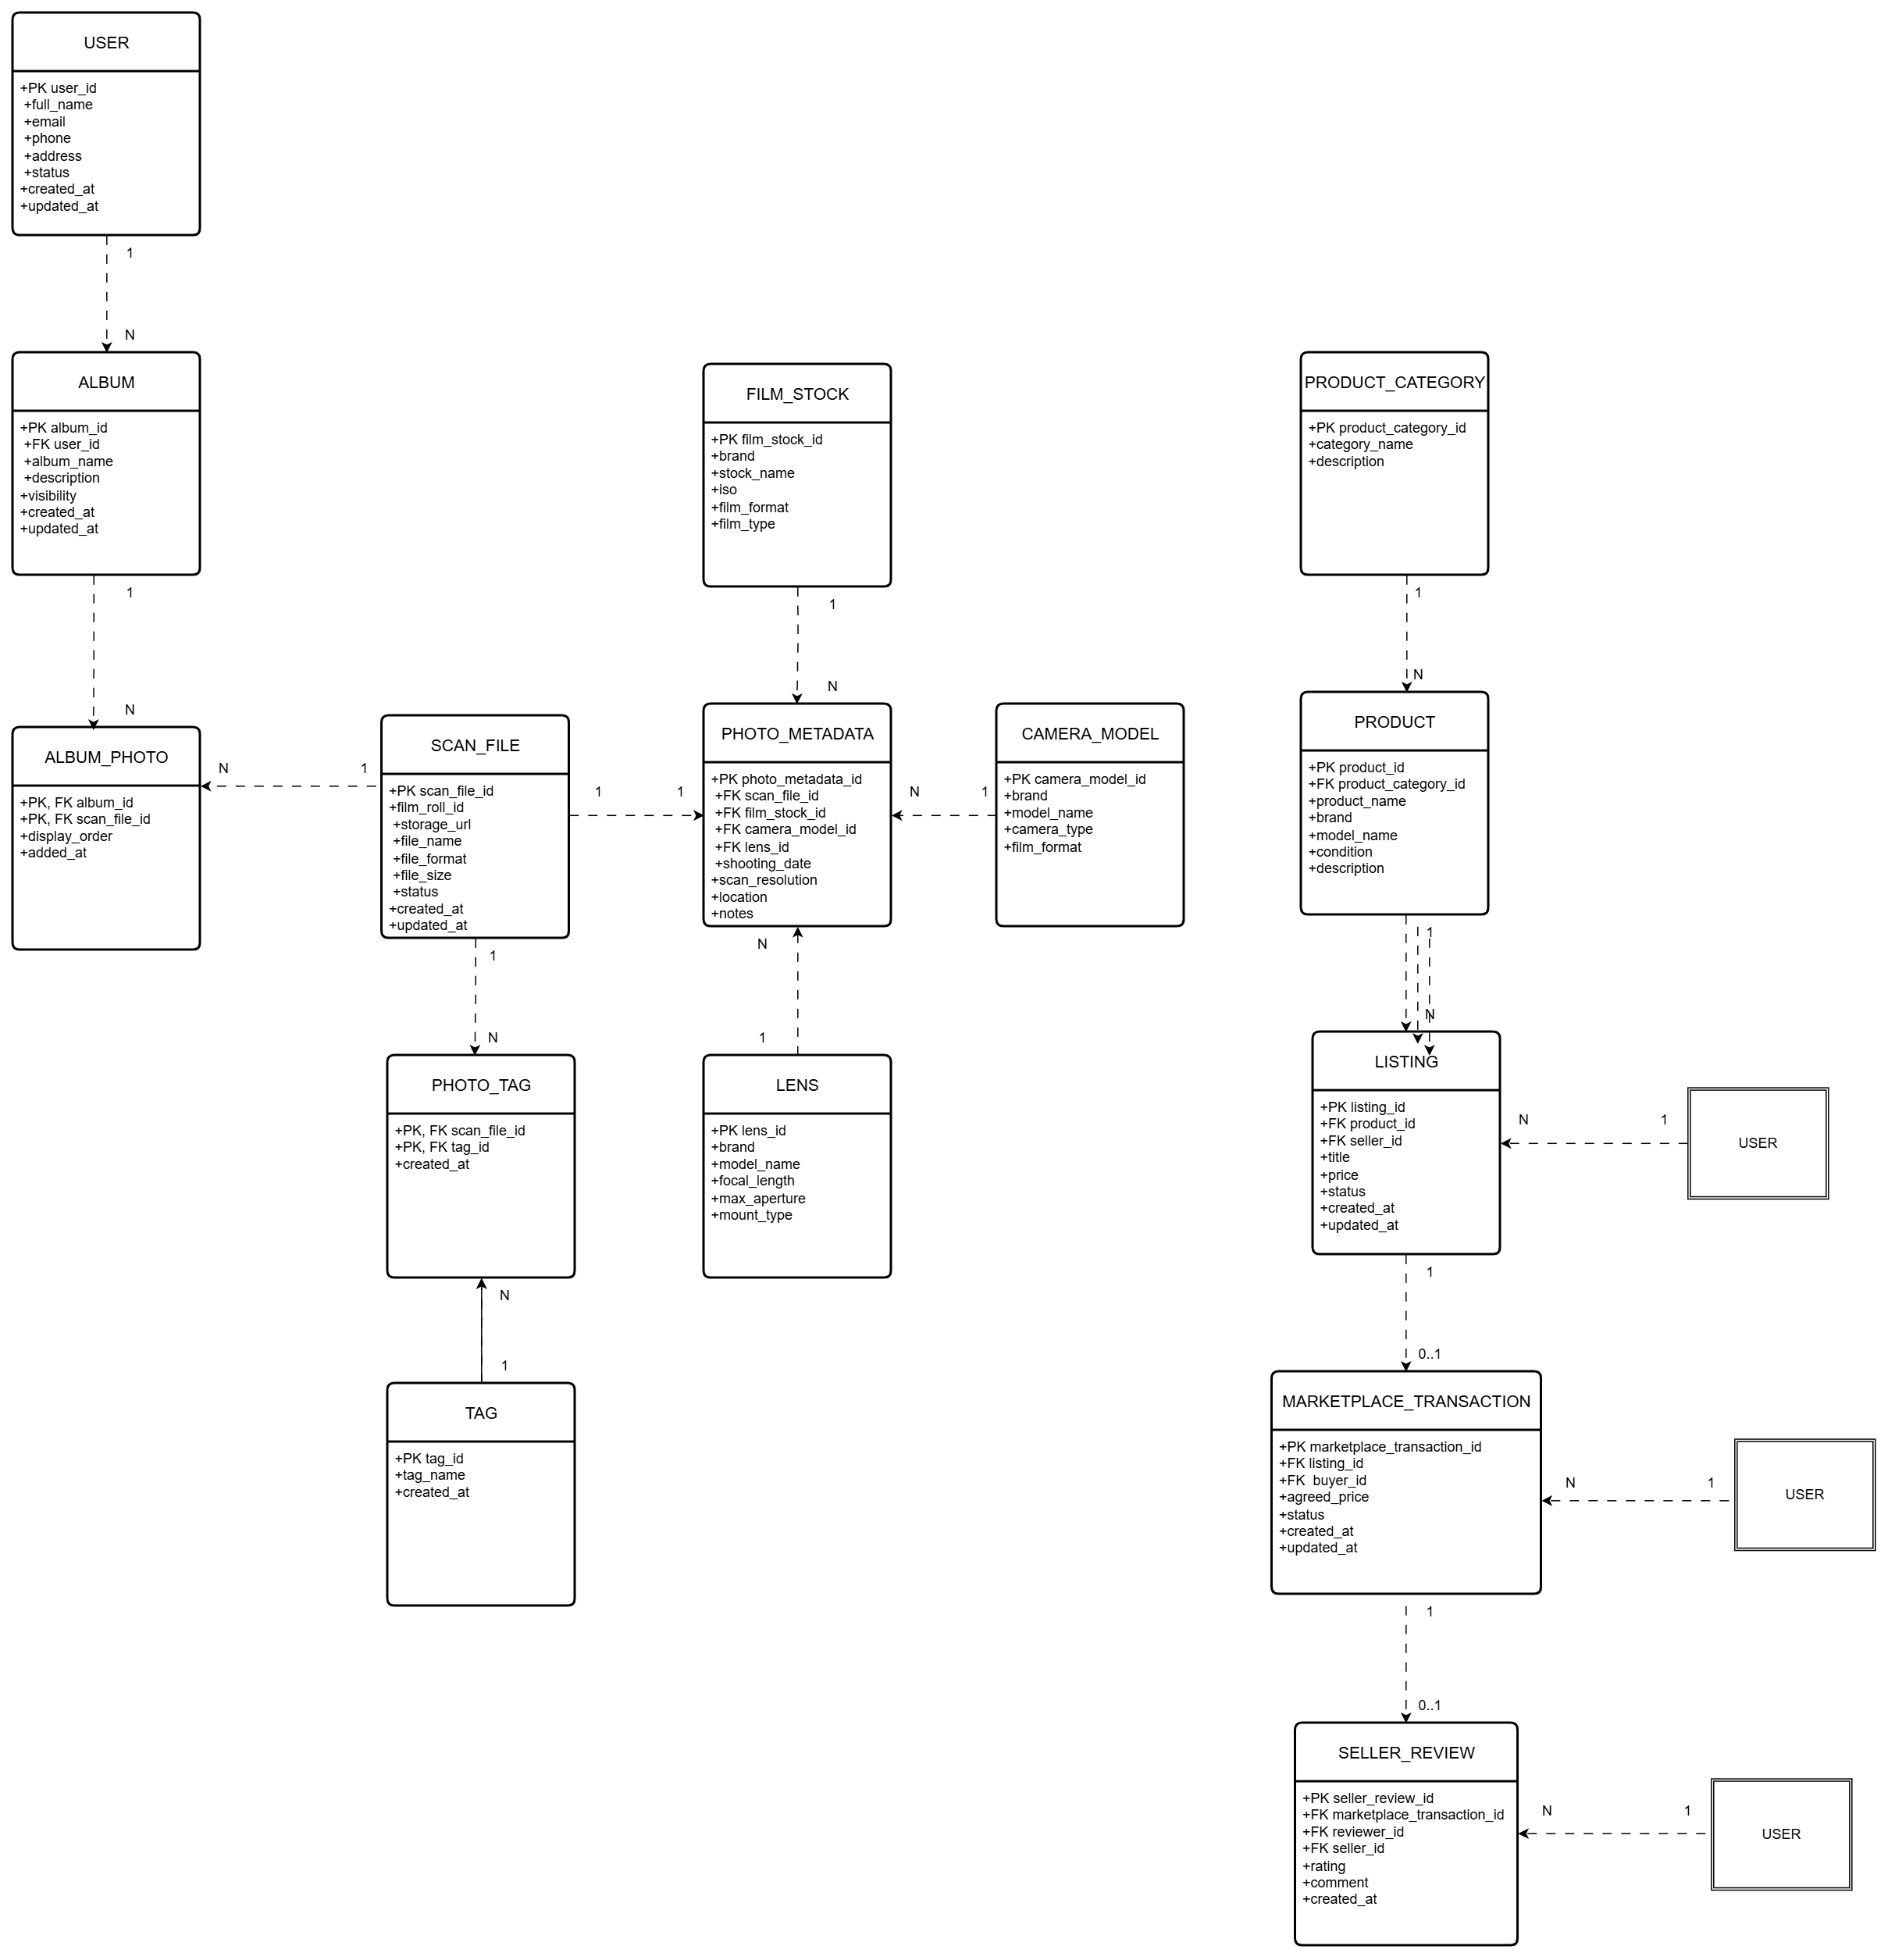
\includegraphics[width=\linewidth,height=0.82\textheight,keepaspectratio]{figures/ERD_P4.png}
    \caption{Sơ đồ thực thể kho ảnh phim số và chợ thiết bị nhiếp ảnh}
    \label{fig:erd-archive-marketplace}
\end{figure}
\clearpage

\section{Tri thức và cộng đồng}

Nhóm thực thể này quản lý bài viết chuyên môn, đánh giá Film Lab và các sự kiện của cộng đồng nhiếp ảnh phim.

\begin{longtable}{p{4cm}p{9.5cm}}
\toprule
\textbf{Thực thể} & \textbf{Mô tả} \\
\midrule
\endhead
\entity{article_categories} & Lưu danh mục phân loại nội dung và kiến thức nhiếp ảnh. \\
\entity{articles} & Lưu bài viết, hướng dẫn và nội dung chia sẻ của cộng đồng. \\
\entity{lab_reviews} & Lưu điểm số và nhận xét của người dùng dành cho Film Lab. \\
\entity{community_events} & Lưu thông tin workshop, photowalk và các sự kiện cộng đồng. \\
\bottomrule
\end{longtable}

\section{Tương tác và hỗ trợ AI}

Nhóm thực thể này ghi nhận hành vi sử dụng và lịch sử trao đổi với trợ lý AI để phục vụ tìm kiếm và gợi ý.

\begin{longtable}{p{4cm}p{9.5cm}}
\toprule
\textbf{Thực thể} & \textbf{Mô tả} \\
\midrule
\endhead
\entity{user_interactions} & Lưu các hành vi tương tác của người dùng với nội dung và chức năng trên nền tảng. \\
\entity{ai_chat_log} & Lưu câu hỏi, câu trả lời và ngữ cảnh trong các cuộc trao đổi với trợ lý AI. \\
\bottomrule
\end{longtable}

\begin{figure}[htbp]
    \centering
    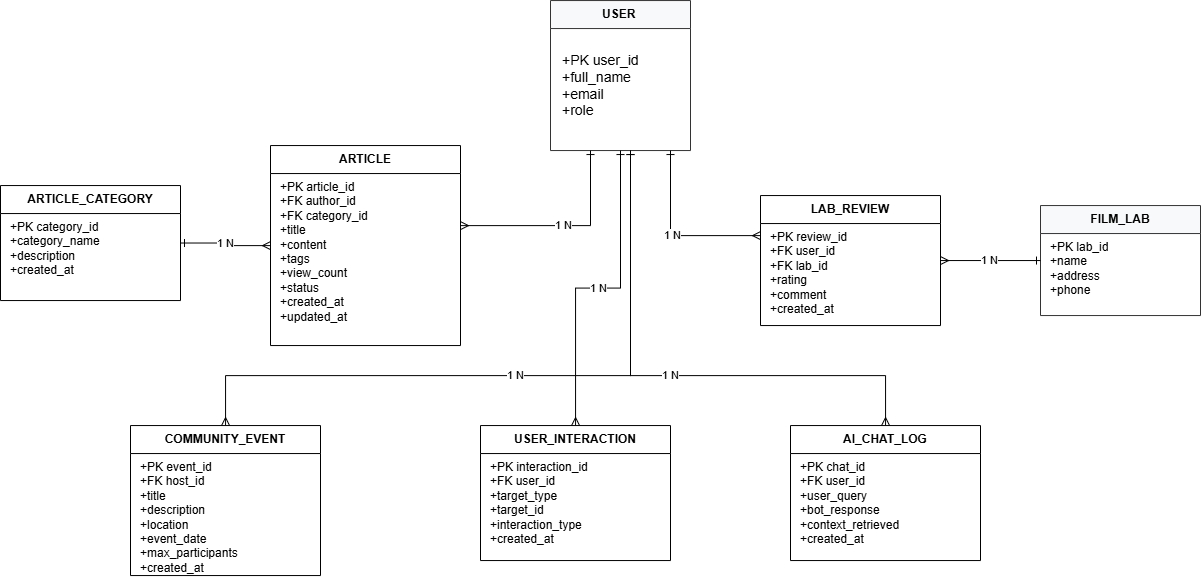
\includegraphics[width=\linewidth,height=0.76\textheight,keepaspectratio]{figures/ERD_P5.png}
    \caption{Sơ đồ thực thể tri thức, cộng đồng, tương tác và hỗ trợ AI}
    \label{fig:erd-community-ai}
\end{figure}
